% $Header: /cvsroot/latex-beamer/latex-beamer/solutions/conference-talks/conference-ornate-20min.en.tex,v 1.6 2004/10/07 20:53:08 tantau Exp $

\documentclass{beamer}

\mode<presentation>
{
%  \usetheme{Hannover}
\usetheme[width=0.7in]{Hannover}
% or ...

  \setbeamercovered{invisible}
  % or whatever (possibly just delete it)
}
\usepackage{longtable}
\usepackage{booktabs}

\usepackage[english]{babel}
% or whatever

\usepackage[latin1]{inputenc}
% or whatever

\usepackage{times}
%\usepackage[T1]{fontenc}
% Or whatever. Note that the encoding and the font should match. If T1
% does not look nice, try deleting the line with the fontenc.
%\usepackage{logictheme}

%\usepackage{hhline}
\usepackage{multirow}
%\usepackage{multicol}
%\usepackage{array}
%\usepackage{supertabular}
%\usepackage{amsmath}
%\usepackage{amsfonts}
\usepackage{totpages}
\usepackage{hyperref}
%\usepackage{booktabs}

%\usepackage{bm}

\usepackage{listings}
\usepackage{color}
 
\definecolor{codegreen}{rgb}{0,0.6,0}
\definecolor{codegray}{rgb}{0.5,0.5,0.5}
\definecolor{codepurple}{rgb}{0.58,0,0.82}
\definecolor{backcolour}{rgb}{0.95,0.95,0.92}
 
\lstdefinestyle{mystyle}{
    backgroundcolor=\color{backcolour},   
    commentstyle=\color{codegray},
    keywordstyle=\color{magenta},
    numberstyle=\tiny\color{codegreen},
    stringstyle=\color{codepurple},
    basicstyle=\tiny,
    breakatwhitespace=false,         
    breaklines=true,                 
    captionpos=b,                    
    keepspaces=true,                 
    numbers=left,                    
    numbersep=5pt,                  
    showspaces=false,                
    showstringspaces=false,
    showtabs=false,                  
    tabsize=2
}
 
\lstset{style=mystyle}
\newcommand{\blt}{- } %used for bullets in a list

\newcounter{datadefnum} %Datadefinition Number
\newcommand{\ddthedatadefnum}{DD\thedatadefnum}
\newcommand{\ddref}[1]{DD\ref{#1}}

\newcommand{\colAwidth}{0.2\textwidth}
\newcommand{\colBwidth}{0.73\textwidth}

\newcommand{\red}{\textcolor{red}}
\newcommand{\ro}[1]{\only<#1>{\red}}

\renewcommand{\arraystretch}{0.6} %so that tables with equations do not look crowded

\pgfdeclareimage[height=0.7cm]{logo}{McMasterLogo}
\title[\pgfuseimage{logo}]  % (optional, use only with long paper titles)
{PhD Committee Meeting \#4}

%\subtitle
%{Include Only If Paper Has a Subtitle}

\author[Slide \thepage~of \pageref{TotPages}] % (optional, use only with lots of
                                              % authors)
{Dan Szymczak}
% - Give the names in the same order as the appear in the paper.
% - Use the \inst{?} command only if the authors have different
%   affiliation.

\institute[McMaster University] % (optional, but mostly needed)
{
  Computing and Software Department\\
  Faculty of Engineering\\
  McMaster University
}
% - Use the \inst command only if there are several affiliations.
% - Keep it simple, no one is interested in your street address.

\date[June 28, 2018] % (optional, should be abbreviation of conference name)
{June 28, 2018}
% - Either use conference name or its abbreviation.
% - Not really informative to the audience, more for people (including
%   yourself) who are reading the slides online

% If you have a file called "university-logo-filename.xxx", where xxx
% is a graphic format that can be processed by latex or pdflatex,
% resp., then you can add a logo as follows:

%\pgfdeclareimage[height=0.5cm]{Mac-logo}{McMasterLogo}
%\logo{\pgfuseimage{Mac-logo}}

% Delete this, if you do not want the table of contents to pop up at
% the beginning of each subsection:
\AtBeginSubsection[]
{
  \begin{frame}<beamer>
    \frametitle{Outline}
    \tableofcontents[currentsection,currentsubsection]
  \end{frame}
}

% If you wish to uncover everything in a step-wise fashion, uncomment
% the following command: 

%\beamerdefaultoverlayspecification{<+->}

\beamertemplatenavigationsymbolsempty 

\begin{document}

%%%%%%%%%%%%%%%%%%%%%%%%%%%%%%%%%%%%%%
\begin{frame}

\titlepage

\end{frame}

%%%%%%%%%%%%%%%%%%%%%%%%%%%%%%%%%%%%%%

\begin{frame}

\frametitle{Overview}
\tableofcontents
% You might wish to add the option [pausesections]

\end{frame}

%%%%%%%%%%%%%%%%%%%%%%%%%%%%%%%%%%%%%%

\section[Recap]{Research Recap}

%%%%%%%%%%%%%%%%%%%%%%%%%%%%%%%%%%%%%%

\begin{frame}
\frametitle{Research Topic Recap}
\framesubtitle{\alt<6->{\ro{6}{KBSE \& The Drasil Framework}}{Motivation -- See 
handout for examples}}

\only<6->{\ro{6}{A Knowledge-Based Software Engineering Approach}}
\begin{itemize}
	\item<1->\alt<7->{\ro{7}{Single knowledge-base}}{Too much 
	duplication!}
	\item<2->\alt<8->{\ro{8}{Guaranteed consistency}}{Inter-/intra-artifact 
	consistency 
	issues}% \& improve:
%		\begin{itemize}
%			\item Verifiability
%			\item Maintainability
%			\item Reusability
%		\end{itemize}
	\item<3->\alt<9->{\ro{9}{Easy to mix and match}}{Design for change} 
	%Easily switch between software family members
	\item<4->\alt<10->{\ro{10}{Reusable across projects}}{Promote reusability}
	\item<5->\alt<11->{\ro{11}{Generate artifacts}}{(Re-)Certification is 
	expensive} 
\end{itemize}

\end{frame}

%%%%%%%%%%%%%%%%%%%%%%%%%%%%%%%%%%%%%%

\begin{frame}
\frametitle{Research Topic Recap}
\framesubtitle{KBSE \& The Drasil Framework}

\only<1-2>{Drasil -- Towards generating Software Families}

\only<1>{
\begin{center}
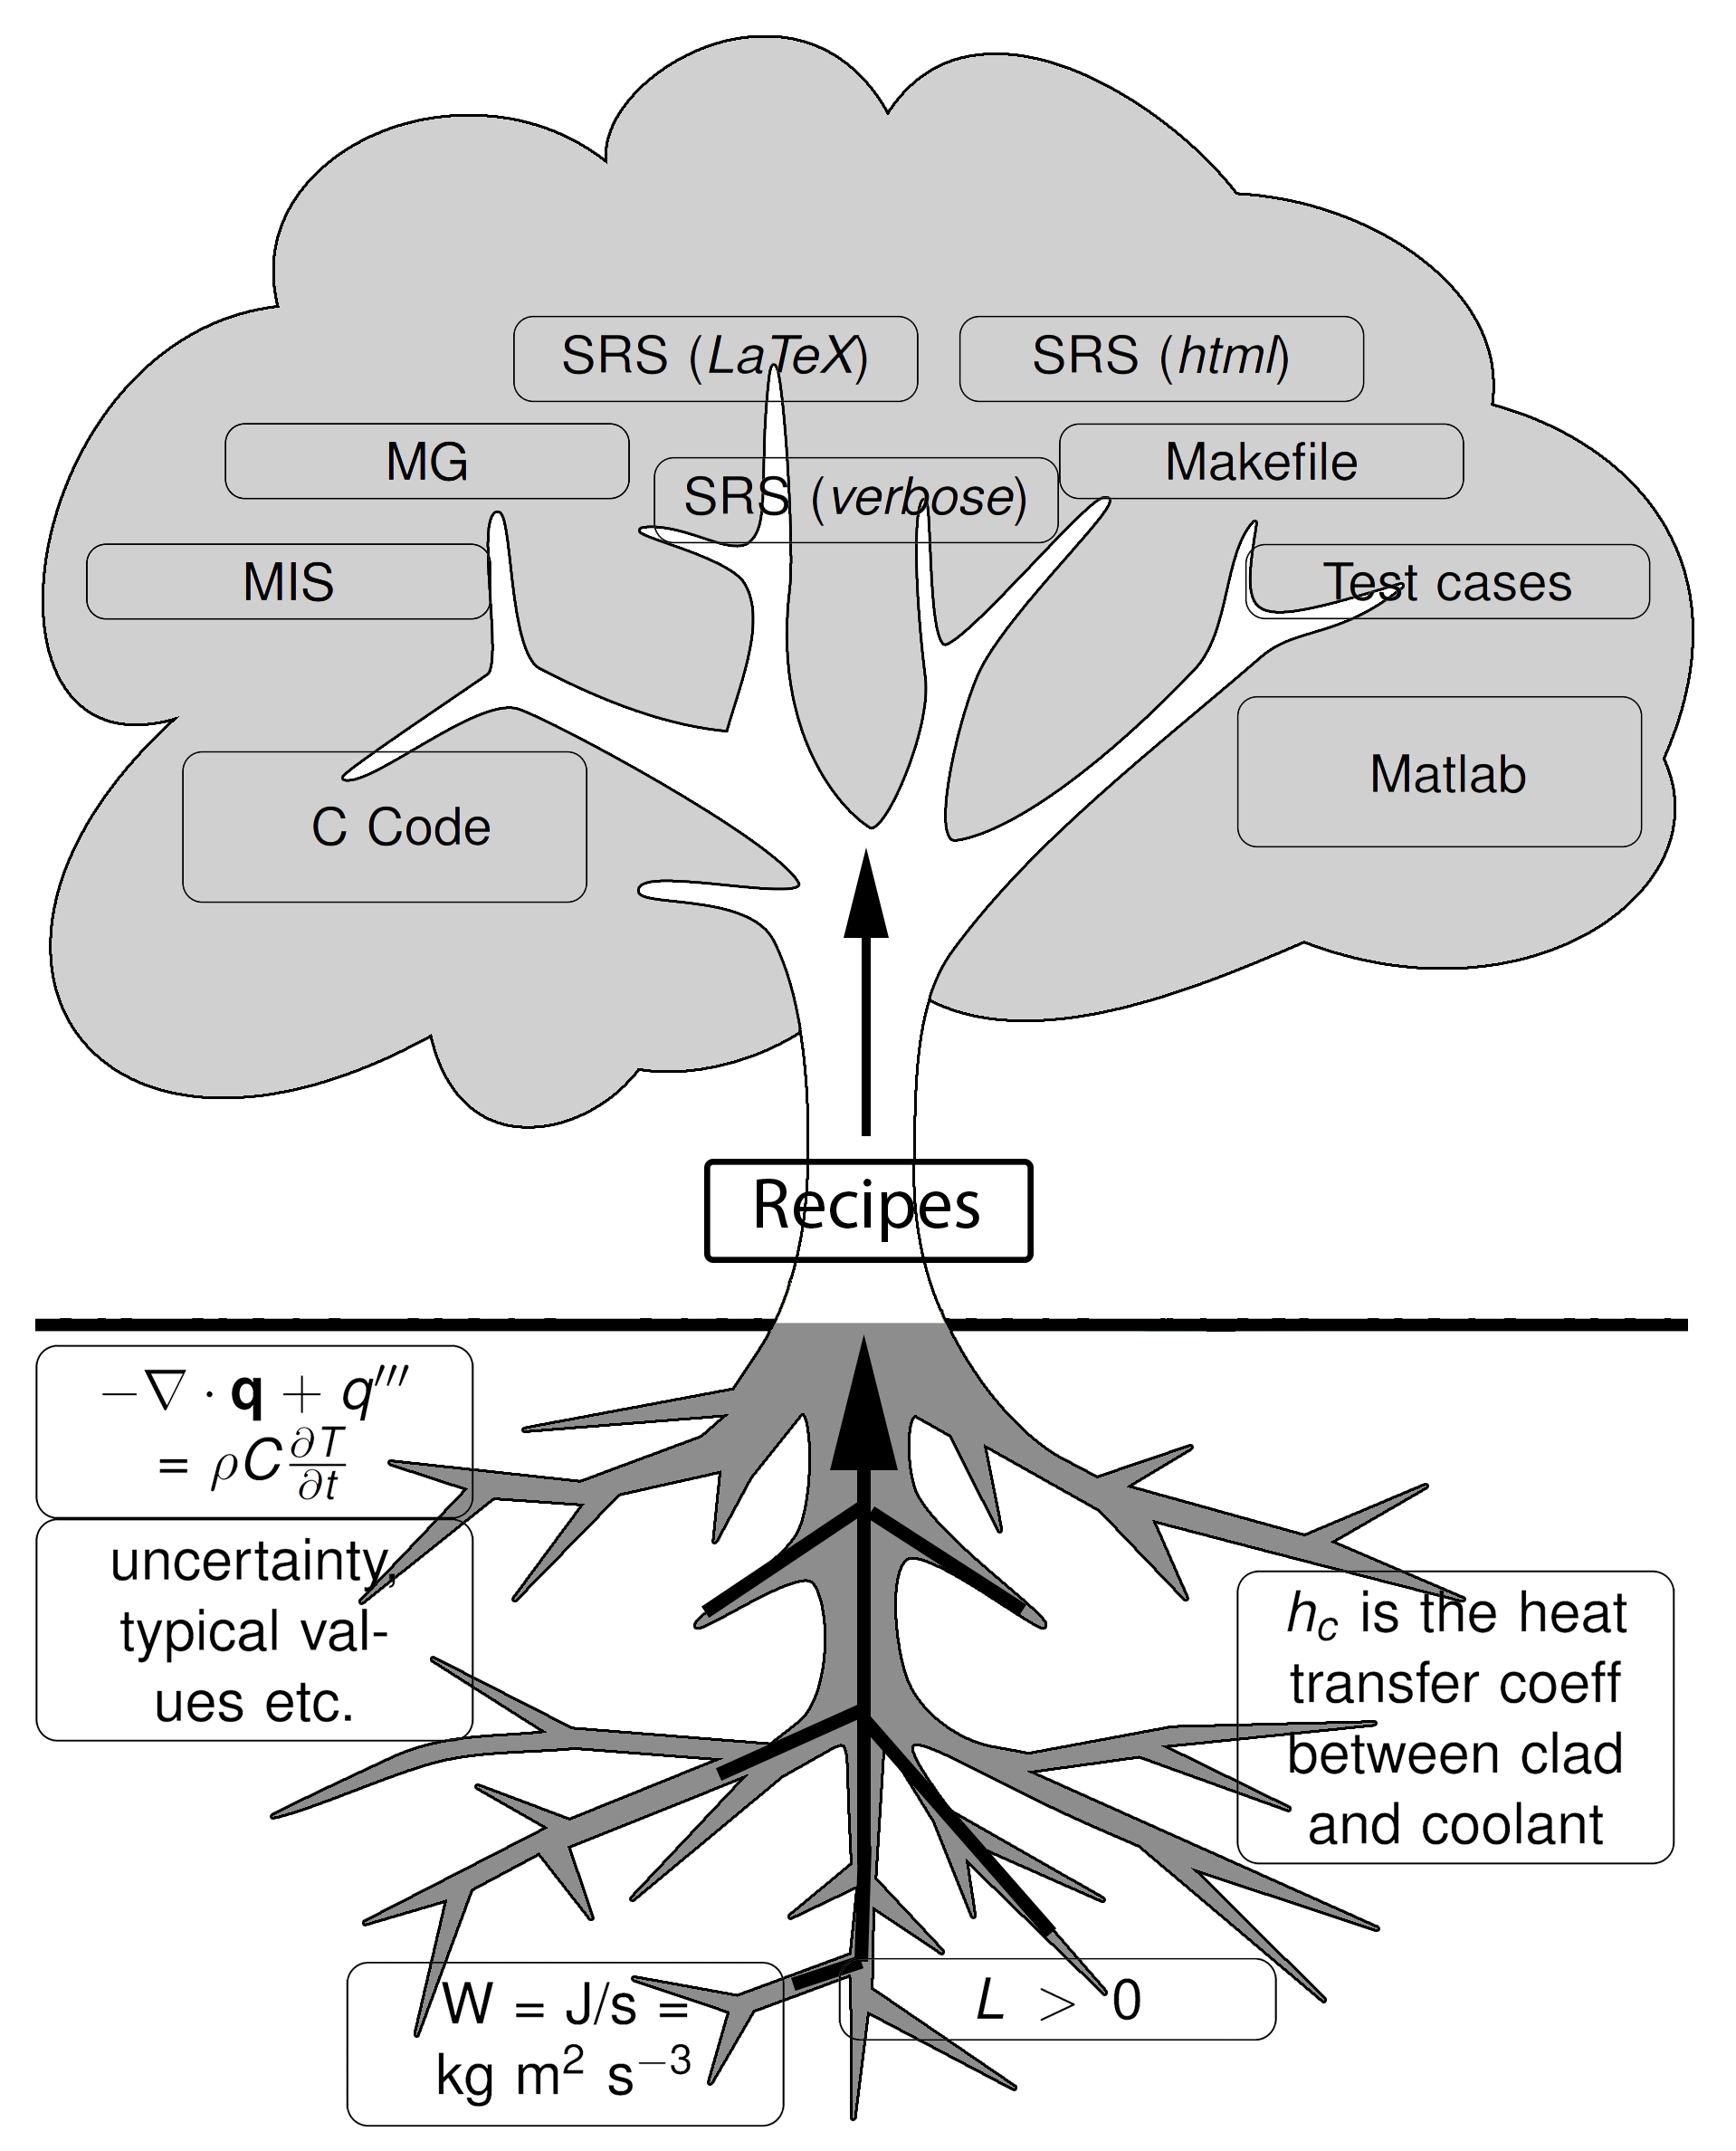
\includegraphics[scale=0.07]{tree.png}
\end{center}
}

\only<2>{
\begin{itemize}
	\item One ``source'', multiple views
	\item Full traceability
	\item Consistent-by-construction artifacts* % does not mean correct
\end{itemize}
}

\only<3>{
Drasil composed of many Domain-Specific Languages (DSLs) including, but not 
limited to:
\begin{itemize}
\item Knowledge Capture
\item Recipes (Document generation)
\item Code Generation
\end{itemize}
}
\end{frame}

%%%%%%%%%%%%%%%%%%%%%%%%%%%%%%%%%%%%%%%

\section[Progress]{Current Progress}

%%%%%%%%%%%%%%%%%%%%%%%%%%%%%%%%%%%%%%%

\begin{frame}

\frametitle{Current Program Progress}
\framesubtitle{A brief overview \only<2>{continued}}

\only<1>{
\begin{itemize}
\item Completed all necessary graduate courses \& comprehensive examinations
%	\begin{itemize}
%	\item CAS781 -- Category Theory: A (11)
%	\item CAS703 -- Software Design: A (11)
%	\item CAS708 -- Scientific Computation: A+ (12)
%	\item CAS761 -- Generative Programming: A+ (12)
%	\end{itemize}

\item Currently Writing:
	\begin{itemize}
	\item Journal paper for ACM TOSEM
	%	\begin{itemize}
	%		\item Focus on (re-)certification and consistency
	%	\end{itemize}
	\item Thesis
	\end{itemize}
\end{itemize}
}

\only<2>{

Research Project: Drasil proof-of-concept ``complete"
\begin{itemize}
	\item Scoped-down due to nature of project
	\item Generating SRS for six case studies \& code for one
	\item Still improving with the help of summer students
% Work still being done is 2-part:
% 1. (Obv) For future researchers/students
% 2. To help me write -- If I can't explain something well-enough, it's usually 
%		because the code needs work
\end{itemize}

}
\end{frame}

%%%%%%%%%%%%%%%%%%%%%%%%%%%%%%%%%%%%%%

\begin{frame}

\frametitle{Since Last Time}
\only<1>{

\framesubtitle{General}
Summer 2017: Supervised 5 research students
\begin{itemize}
\item Cleaned up case studies
\item Helped improve Drasil
\end{itemize}

Submitted to SE-CoDeSE'17 -- Rejected

Began a paper for FASE 2018 -- Scrapped

Met with OPG -- Positive feedback

Co-supervising 3 research students

Writing %mentioned earlier
}

\only<2>{
\framesubtitle{Drasil-Specific}

Total of 372 issues closed on the Drasil github

\begin{itemize}
\item Haddock % Automated generation of some Drasil user-documentation using 
%Haddock
\item Chunk and referencing databases %improved referencing
\item Improved the Drasil class hierarchy %Added to, and refactored, 
% Citations, Theories, Labels, etc.
\item Finished creating Document Language (Cont'd)
\item Continuous Integration \& automated tests
\item General source clean-up and refactoring % template haskell
\end{itemize}

Currently $\sim$130 open issues guiding development
}
\end{frame}

%%%%%%%%%%%%%%%%%%%%%%%%%%%%%%%%%%%%%%%

\section[Results]{Results to date}

%%%%%%%%%%%%%%%%%%%%%%%%%%%%%%%%%%%%%%%

\begin{frame}
\frametitle{Results}
\framesubtitle{Document Language}

\only<1>{
Introduction of new Document Language led to:
\begin{itemize}
\item De-embedding English
\item More readable source %debatable
\item Improved sanity checking
\end{itemize}
}

\only<2>{
\framesubtitle{Old}

\lstinputlisting[language=Haskell, firstline=46, lastline=74]{BodyOld.hs}

}

\only<3->{
\framesubtitle{\only<3>{New}\only<4>{140 ``Old" line equiv.; 260 (216 
gen.) lines of TeX}} %793 generated lines of HTML / >800 manual
\only<3>{\lstinputlisting[language=Haskell, firstline=92, 
lastline=119]{BodyNew.hs}}
\only<4>{\lstinputlisting[language=Haskell, firstline=92, 
lastline=102, frame=single]{BodyNew.hs}
\lstinputlisting[language=Haskell, firstline=103, 
lastline=119, firstnumber=12]{BodyNew.hs}}
}


\end{frame}

%%%%%%%%%%%%%%%%%%%%%%%%%%%%%%%%%%%%%

\begin{frame}[fragile]
\frametitle{Results}
\framesubtitle{Sanity Checking}

SSP Example (Issue \#348)

\begin{minipage}{.4\linewidth}
\begin{equation}
S_i = \frac{P_i}{FS}
\end{equation}
\end{minipage}%
\begin{minipage}{.4\linewidth}
\begin{equation}
FS = \frac{S_i}{\ro{2}{\tau{}_i}}
\end{equation}
\end{minipage}

\only<2->{

\vspace{.5cm}Where did \ro{2}{$\tau{}_i$} come from?\vspace{.3cm}

Were $S_i$ and $P_i$ swapped?
}

\only<3>{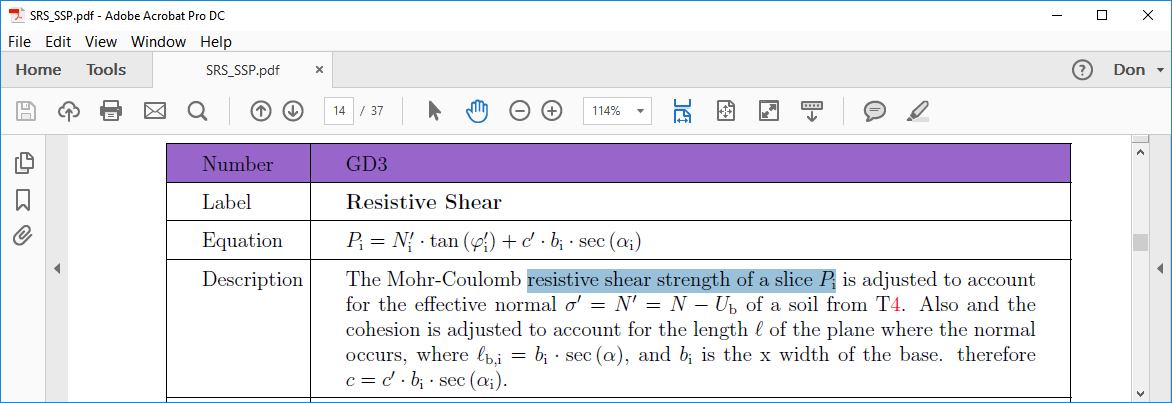
\includegraphics[width=\textwidth]{Pi.png}}
\only<4>{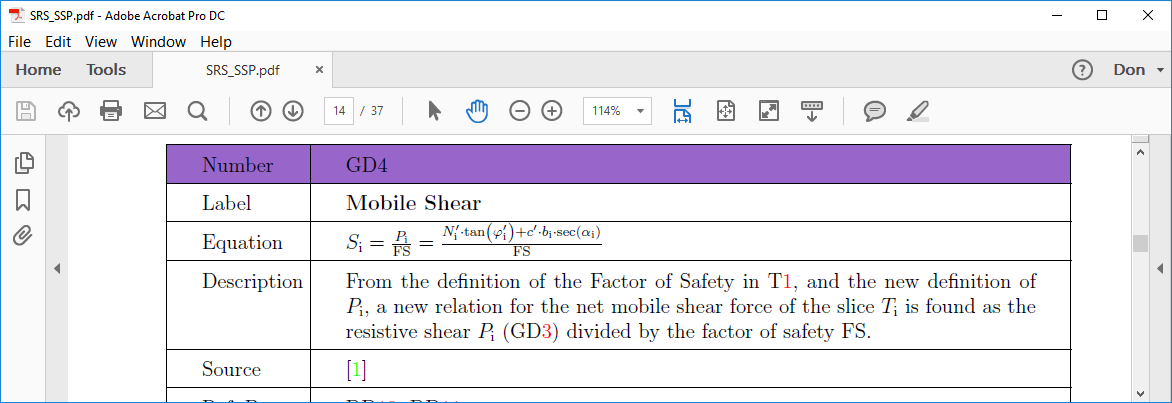
\includegraphics[width=\textwidth]{Si.png}}
\only<5>{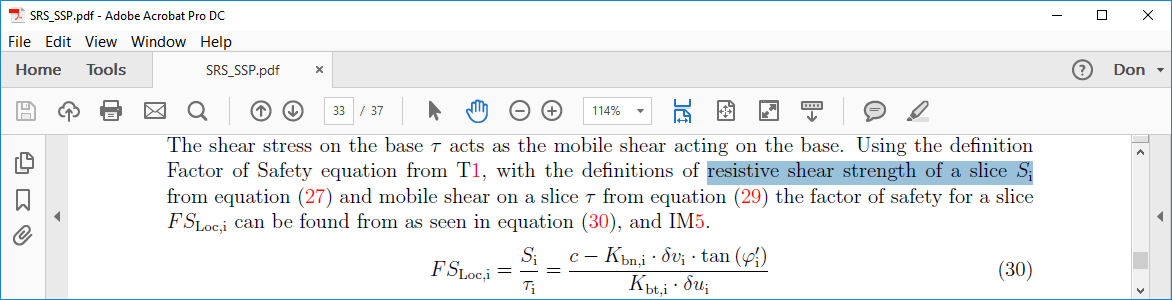
\includegraphics[width=\textwidth]{taui.png}}

\only<6->{

\begin{itemize}
\item $\tau{}_i$ was not defined anywhere in the documents
\item Found with Drasil -- undefined symbols throw errors
\item Equation based on concepts -- symbols automatically retrieved
\end{itemize}
}
%Original issue was a bit more complicated, but came down to this.

\end{frame}

%%%%%%%%%%%%%%%%%%%%%%%%%%%%%%%%%%%%%

\begin{frame}

\frametitle{Results} %DS Get a better name for this
\framesubtitle{Conceptual Inconsistencies in Software Artifacts}

Manually created artifacts are human-readable.

Problems arise when explaining things to a machine.

\begin{itemize}
\item What do our artifacts \emph{mean}?
\item What is each section contributing? %(in an artifact) --> New knowledge 
%(assumps, reqs)? Building off previous towards a solution?
\item Why do we organize things a given way?
%\item Are models/definitions different? How?
\end{itemize}

Need to be more rigorous!

\end{frame}

%%%%%%%%%%%%%%%%%%%%%%%%%%%%%%%%%%%%%%

\section[Next Steps]{Next Steps}

%%%%%%%%%%%%%%%%%%%%%%%%%%%%%%%%%%%%%%

\begin{frame}

\frametitle{Next Steps for Me}
\framesubtitle{Broad Strokes}


\begin{Large}
What next?
\end{Large}

\begin{itemize}
\item Finish writing paper for ACM TOSEM
\item Complete Thesis writing
\item Continue improving Drasil %issues
\end{itemize}
\end{frame}

%%%%%%%%%%%%%%%%%%%%%%%%%%%%%%%%%%%%%%

\begin{frame}
\frametitle{Summary}

Problem:
\begin{itemize}
\item Duplication
\item Inconsistency
\item Design for change
\item Promote re-usability
\item Re-certification
\end{itemize}

\emph{Solution}:
\begin{center}
Capture fine-grained knowledge \& generate \ro{1}{ALL} artifacts
\end{center}


\end{frame}

%%%%%%%%%%%%%%%%%%%%%%%%%%%%%%%%%%%%%%

\end{document}
